\section{要素技術}\label{sec:要素技術}
\tikzset{str/.style  args={#1with#2}{rounded corners, minimum height=.7cm,align=center,text width=#1,fill=#2}}
\subsection{仮想マシン}
仮想化は,辞書で以下のように説明されている.
\begin{quote}
    ``コンピューターの物理的資源を論理的に分割して,それぞれ独立並列した状態で利用できるようにすること。1台のサーバーで,複数の基本ソフトを独立並列に動作させるサーバー仮想化など。''  \hfill\cite{スーパー大辞林}
\end{quote}
仮想マシン(Virtual Machine)は,辞書で以下のように説明されている.
\begin{quote}
    ``あるコンピューターシステムの動作を,別システムで再現するソフトウエア。また,そのような動作環境。あるOSの動作を別の OS 上で再現する場合など。バーチャルマシン。VM。''\hfill\cite{スーパー大辞林}
\end{quote}
つまり,1台の計算機で複数のOSやアプリケーションなどを並列に動作させる,仮想化を実現するためのソフトウェアや動作環境のことを「仮想マシン」と呼んでいる.
今回は「ホスト型」と「ハイパーバイザ型」の仮想化について説明する.

\begin{wrapfigure}{r}[0mm]{.3\textwidth}
    \centering
    \begin{tikzpicture}
        \node[str=.28\textwidth with gray!60](hw){ハードウェア};
        \node[str=.28\textwidth with gray!50,above=.1cm of hw](hos){ホストOS};
        \node[str=.28\textwidth with gray!40,above=.1cm of hos](hsw){ホスト型仮想化ソフトウェア};
        \node[str=.13\textwidth with gray!30,above=.1cm of hsw.north west,anchor=south west](gos1){ゲストOS};
        \node[str=.13\textwidth with gray!30,above=.1cm of hsw.north east,anchor=south east](gos2){Linux};
        \node[str=.055\textwidth with gray!20,above=.1cm of gos1.north west,anchor=south west](sw1){\tiny App};
        \node[str=.055\textwidth with gray!20,above=.1cm of gos1.north east,anchor=south east](sw2){\tiny App};
        \node[str=.055\textwidth with gray!20,above=.1cm of gos2.north west,anchor=south west](sw3){\tiny Apache};
        \node[str=.055\textwidth with gray!20,above=.1cm of gos2.north east,anchor=south east](sw4){\tiny Python};
    \end{tikzpicture}
    \caption{ホスト型}
    \label{fig:ホスト型}
    \vspace{-1cm}
\end{wrapfigure}
\subsubsection*{ホスト型}
ホスト型の仮想化は,「ホスト型仮想化ソフトウェア」を用いて仮想化する手法である(\figref{fig:ホスト型}).
ホスト型の仮想化メリットは,ホスト型仮想化ソフトウェアが扱いやすい点にある.代表的なものとしてVirtualBoxがある.\par
ホスト型仮想化のメリットとして挙げられるのが,既存OSを利用できる点である.それに対して,ホストOSを動作させるためのリソースが必要になり,物理サーバはもちろん,後述するハイパーバイザ型に比べても性能が劣る\cite{itmanage}.

\begin{wrapfigure}{r}[0mm]{.3\textwidth}
    \centering
    \begin{tikzpicture}
        \node[str=.28\textwidth with gray!60,](hw){ハードウェア};
        \node[str=.28\textwidth with gray!45,above=.1cm of hw](hpv){ハイパーバイザ};
        \node[str=.13\textwidth with gray!30,above=.1cm of hpv.north west,anchor=south west](gos1){ゲストOS};
        \node[str=.13\textwidth with gray!30,above=.1cm of hpv.north east,anchor=south east](gos2){Linux};
        \node[str=.055\textwidth with gray!20,above=.1cm of gos1.north west,anchor=south west](sw1){\tiny App};
        \node[str=.055\textwidth with gray!20,above=.1cm of gos1.north east,anchor=south east](sw2){\tiny App};
        \node[str=.055\textwidth with gray!20,above=.1cm of gos2.north west,anchor=south west](sw3){\tiny Apache};
        \node[str=.055\textwidth with gray!20,above=.1cm of gos2.north east,anchor=south east](sw4){\tiny Python};
    \end{tikzpicture}
    \caption{ハイパーバイザ型}
    \label{fig:ハイパーバイザ型}
    \vspace{-1cm}
\end{wrapfigure}

\subsubsection*{ハイパーバイザ型}
ホストOSを必要としない,「ハイパーバイザ」と呼ばれる仮想化ソフトウェアを用いた仮想化(\figref{fig:ハイパーバイザ型}).
ホストOSを必要としないので,ホスト型と比べてリソースの使用効率が良い.
このハイパーバイザ型には,「準仮想化」と「完全仮想化」の2種類が存在する.
\begin{description}
    \setlength{\leftskip}{1em}
    \item[完全仮想化] ハードウェアも含めて仮想化する方式.
        ユーザモードで動作するゲストOSから{{特権命令を実行した}}とき,必要に応じてハイパーバイザへ処理を移行する.
        ``ユーザモードで動作するゲストオペレーティングシステムは,自分の動作している環境(仮想化であるかないか)をまったく意識する必要がないため,完全仮想化と呼ばれている.''\cite[p.159]{オペレーティングシステム}
        この方式は,特権命令をハイパーバイザへ移行して処理するので,オーバーヘッドが大きく,ハイパーバイザも特権命令の実行を常時監視する必要がある.
\end{description}

\begin{description}
    \setlength{\leftskip}{1em}
    \item[準仮想化] 仮想マシンからハードウェアを直接操作できるように,ゲストOSを改変した方式.
        完全仮想化に比べてオーバーヘットが激減するが,OSの書き換えが必要であるため,すべてのOSには対応できない.
\end{description}
\subsubsection*{仮想化の利点と欠点}
仮想化は,リソースの集約に役立つ技術である.
1台のサーバ上に複数の仮想環境を作ることで,初期コスト,管理コストの削減ができ,リソースを集約することで管理が簡便になる.\par
ただし,物理{{サーバ}}に比べて性能が劣り,リソースを集約していることで,ハードウェアの故障による障害範囲が広くなる.
\subsection{スケールインとスケールアウト}
クラウドでは,仮想サーバのスペック(CPUやメモリサイズなど)や台数の変更によるサーバリソースの調節が簡便にできる.
スケールインとスケールアウトは,仮想サーバのリソース調節における分類である.
\begin{description}
    \item[スケールアップ] サーバのスペックが不足しているときに,仮想サーバのスペックを上げること.
    \item[スケールダウン] サーバスペックが過剰であるときに,仮想サーバのスペックを下げること.
    \item[スケールアウト] 同じようなスペックのサーバを複数台並べて,最適なリソース量を提供すること.
    \item[スケールイン] リクエストに対して,{{サーバ}}台数が過剰であるとき,{{サーバ}}の台数を減らして最適なリソース量を提供すること.\hfill\cite{スケールアップ}
\end{description}
\begin{figure}[htbp]
    \centering
    \begin{minipage}[b]{.23\textwidth}
        \centering
        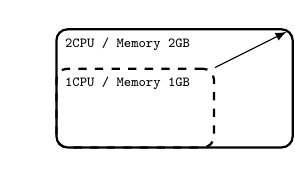
\begin{tikzpicture}
            \node[draw,dashed,thick,rounded corners,minimum width=2cm,minimum height=1cm](sp1){};
            \node[draw,thick,rounded corners,minimum width=3cm,minimum height=1.5cm,anchor=south west]at(sp1.south west)(sp2){};
            \draw[-latex,shorten >= 1mm](sp1.north east)--(sp2.north east);
            \node[below right]at(sp1.north west){\tiny\ttfamily 1CPU / Memory 1GB};
            \node[below right]at(sp2.north west){\tiny\ttfamily 2CPU / Memory 2GB};
        \end{tikzpicture}
        \caption{スケールアップ}
    \end{minipage}
    \begin{minipage}[b]{.23\textwidth}
        \centering
        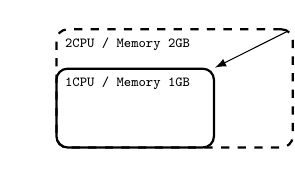
\begin{tikzpicture}
            \node[draw,thick,rounded corners,minimum width=2cm,minimum height=1cm](sp1){};
            \node[draw,dashed,thick,rounded corners,minimum width=3cm,minimum height=1.5cm,anchor=south west]at(sp1.south west)(sp2){};
            \draw[-latex,shorten <= 1mm](sp2.north east)--(sp1.north east);
            \node[below right]at(sp1.north west){\tiny\ttfamily 1CPU / Memory 1GB};
            \node[below right]at(sp2.north west){\tiny\ttfamily 2CPU / Memory 2GB};
        \end{tikzpicture}
        \caption{スケールダウン}
    \end{minipage}
    \begin{minipage}[b]{.23\textwidth}
        \centering
        \begin{tikzpicture}
            \node[minimum width=.5cm,minimum height=1.5cm,anchor=center,draw](sv1){\scriptsize\rotatebox{90}{\ttfamily server}};
            \node[minimum width=.5cm,minimum height=1.5cm,anchor=center,draw,right=.2cm of sv1](sv2){\scriptsize\rotatebox{90}{\ttfamily server}};
            \node[minimum width=.5cm,minimum height=1.5cm,anchor=center,draw,right=.2cm of sv2](sv3){\scriptsize\rotatebox{90}{\ttfamily server}};
        \end{tikzpicture}
        \caption{スケールアウト}
    \end{minipage}
    \begin{minipage}[b]{.23\textwidth}
        \centering
        \begin{tikzpicture}
            \node[minimum width=.5cm,minimum height=1.5cm,anchor=center,draw](sv1){\scriptsize\rotatebox{90}{\ttfamily server}};
            \node[minimum width=.5cm,minimum height=1.5cm,anchor=center,draw,right=.2cm of sv1](sv2){\scriptsize\rotatebox{90}{\ttfamily server}};
            \node[minimum width=.5cm,minimum height=1.5cm,anchor=center,draw,right=.2cm of sv2,gray=10!](sv3){\scriptsize\rotatebox{90}{\ttfamily server}};
        \end{tikzpicture}
        \caption{スケールイン}
    \end{minipage}
\end{figure}
\subsection{IaaS, PaaS, SaaS}
クラウドを利用するとき,クラウド事業者が管理する部分と,クラウド利用者が管理する部分を明確にする必要がある.
IaaS,PasS,SaaSとは,クラウド事業者が管理する部分に対して分類したものである.これを「サービスレイヤ」と呼ぶこともある.
\begin{description}
    \item[SaaS: Software as a Service] アプリケーションソフトウェアをサービスとして提供する.電子メール(Gmail)やオンライン会議システム(Zoom)などがある.
    \item[PaaS: Platform as a Service] ライブラリの利用をサービスとして提供する.ユーザはライブラリを用いてアプリケーションを構成する.提供されているライブラリの管理はクラウド事業者が行うので,ユーザはライブラリを意識する必要がない.代表的なものにストレージサービスのAmazon S3がある.
    \item[IaaS: Infrastructure as a Service] インフラストラクチャ(仮想ハードウェアやネットワーク)をサービスとして提供する.ユーザは提供された仮想ハードウェア上にOSをインストールし,そのうえでアプリケーションなどを動かす.代表的なものにAmazon EC2がある.
\end{description}
\begin{flushright}
    \cite[p.164]{オペレーティングシステム}
\end{flushright}
